\section{Gaussian Mixture Model}%
\label{sec:l2hmc_gmm}
%
The Gaussian Mixture Model (GMM) is a notoriously difficult example for
traditional HMC to sample accurately due to the existence of multiple modes.
%
In particular, HMC cannot mix between modes that are reasonably separated
without recourse to additional tricks.
%
This is due, in part, to the fact that HMC cannot easily traverse the
low-density zones which exist between modes.

In the most general case, we consider a target distribution described by a
mixture of $M > 1$ components in
$\mathbb{R}^{D}$ for $D \geq 1$:
%
\begin{equation}
    p(\mathbf{x}) \equiv \sum_{m=1}^{M} p(m) p(\mathbf{x}|m) \equiv
        \sum_{m=1}^{M} \pi_m p(\mathbf{x}|m) \quad \forall \,\,\mathbf{x} \in
        \mathbb{R}^{D}
    \label{eq:gmm_model}
\end{equation}
%
where $\sum_{m=1}^{M} \pi_m = 1$, $\pi_M \in (0, 1)$ $\forall m = 1, \ldots, M$
and each component distribution is a normal probability distribution in
$\mathbb{R}^{D}$.
%
So $\mathbf{x}|m \sim \mathcal{N}(\bm{\mu}_m, \bm{\Sigma}_m)$, where
$\bm{\mu}_m \equiv \mathbb{E}_{p{(\mathbf{x}|m)}}\left\{\mathbf{x}\right\}$ and
$\mathbf{\Sigma}_m \equiv \mathbb{E}_{p{(\mathbf{x}|m)}}{\left\{{(\mathbf{x} -
\bm{\mu}_m)}{(\mathbf{x} - \bm{\mu}_m)}^{T}\right\}} > 0$ are the mean vector
and covariance matrix, respectively, of component $m$.
%%%%%%%%%%%%%%%%%%%%%%%%%%%%%%%%%%%%%%%%%%%%%%%%%%%%%%%%%%%%%%%%%%%%%%%%%%%%%%%
%
%%%%%%%%%%%%%%%%%%%%%%%%%%%%%%%%%%%%%%%%%%%%%%%%%%%%%%%%%%%%%%%%%%%%%%%%%%%%%%%
\subsection{Example}
%
Consider a simple 2D case consisting of two Gaussians 
%
\begin{equation}
    \mathbf{x} \sim \pi_1 \,\mathcal{N}(\bm{\mu}_1, \bm{\Sigma}_1) +
        \pi_2\, \mathcal{N}(\bm{\mu}_2, \bm{\Sigma}_2)
    \label{eq:log_likelihood_example}
\end{equation}
%
with $\pi_1 = \pi_2 = 0.5$, $\bm{\mu}_1 = (-2, 0)$, $\bm{\mu}_2 = (2, 0)$ and
%
\begin{equation}
    \bm{\Sigma}_1 = \bm{\Sigma}_2 = 
        \begin{bmatrix}
            0.1    & 0 \\
            0       & 0.1 
        \end{bmatrix}
    \label{eq:covariance_matrix}
\end{equation}
%
The results of trajectories generated using both traditional HMC and the L2HMC
algorithm can be seen in Fig.~\ref{fig:gmm_trajectories}.
a
Note that traditional HMC performs poorly and is unable to mix between the two
modes, whereas L2HMC is able to correctly sample from the target distribution
without getting stuck in either of the individual modes.

%
The L2HMC sampler was trained using simulated annealing using the schedule
shown in Eq~\ref{eq:gmm_annealing} with a starting temperature of $T = 10$, for
$5,000$ training steps.
%
By starting with a high temperature, the chain is able to move between both
modes (`tunnel') successfully.
%
Once it has learned this, we can lower the temperature back to $T = 1$ and
recover the initial distribution while preserving information about tunneling
in the networks ``memory''.
%
\begin{equation}
  T(n) = {\left(T_{i} - T_{f}\right)} \cdot {\left(1 -
  \frac{n}{N_{\mathrm{train}}}\right)} + T_{f} 
\label{eq:gmm_annealing}
\end{equation}
%
\begin{figure}[htbp]
    \centering
    \includegraphics[width=\textwidth]{gmm_figures/iso_gmm_chains1}
    \caption{Comparison of trajectories generated using L2HMC (top), and
        traditional HMC with $\eps = 0.25$ (middle) and $\eps = 0.5$ (bottom).
        Note that L2HMC is able to successfully mix between modes, whereas HMC
        is not.}%
\label{fig:gmm_trajectories}
\end{figure}
%
\begin{figure}[htbp]
    \centering
    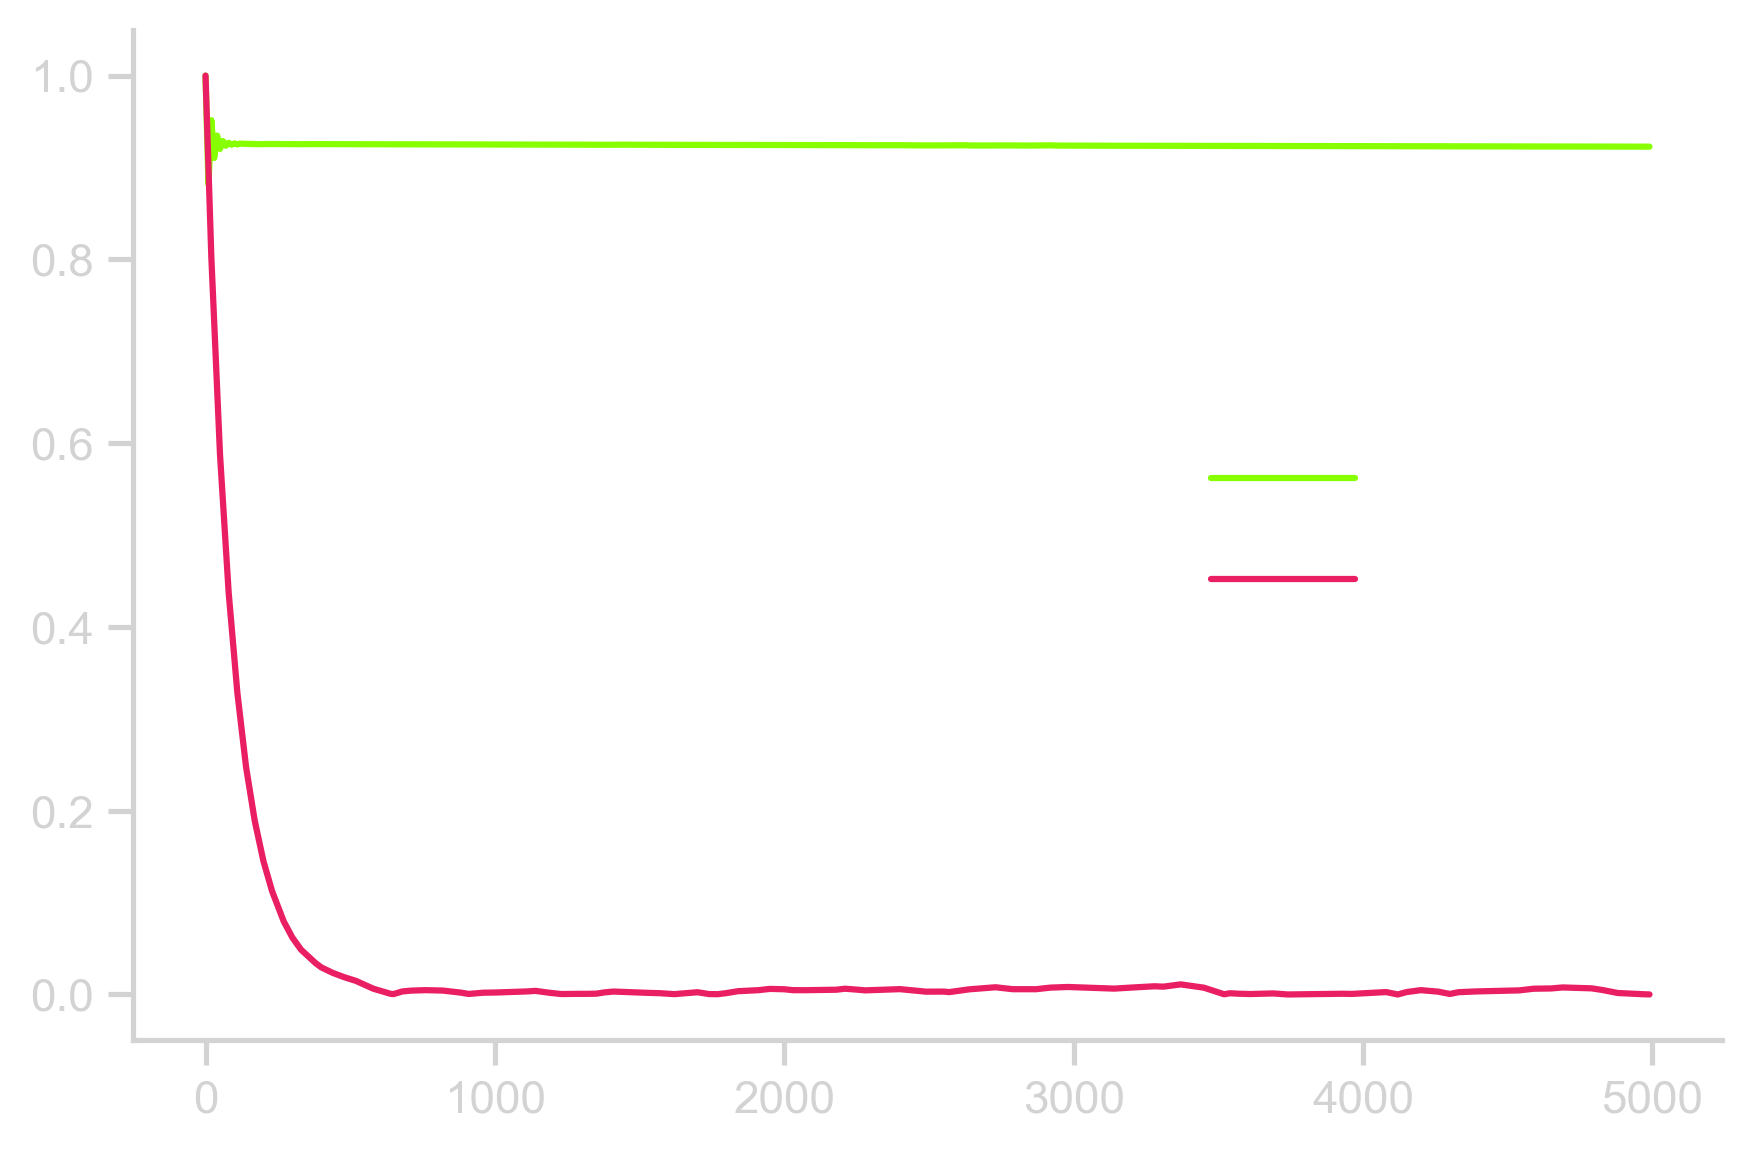
\includegraphics[width=0.98\textwidth]{gmm_figures/gmm_acl}
    \caption{Autocorrelation vs.\ gradient evaluations (i.e.\ MD steps). Note
    that L2HMC (blue) has a significantly reduced autocorrelation after the
  same number of gradient evaluations when compared to either of the two HMC
trajectories}% 
\label{fig:gmm_autocorrelation} 
\end{figure}
%%%%%%%%%%%%%%%%%%%%%%%%%%%%%%%%%%%%%%%%%%%%%%%%%%%%%%%%%%%%%%%%%%%%%%%%%%%%%%%
%
